% STATUS: ACTIVE | CONDENSED 5-STATE PRESENTATION COPY (2026-08-31)
%   Copied from formC_state_b.tex @ HEAD (pre-2026-08-30 five-state writing) on
%   user request: complete definitions, five states only (no MA(2) memory
%   states -- the white-container Q33 carries the full Var(eps_w) instead),
%   no Seed-and-prior section, no result figures, no c(w)/C_dpmr/C_n and no
%   f_R (user request 2026-08-31): a_bar is defined by a/a_nom alone, kappa_T
%   is taken as the primitive thermal constant, and the readout-chain
%   constants (IF_var, xi) are given as four offline pure numbers instead of
%   being expanded through C_dpmr/C_n. R2 carries the production whitening
%   factor 2*a_cov^2; its delay term a_cov^2*d*Q44 is dropped (below 1e-4 of
%   R2 everywhere on the canonical band). Everything is written AT THE
%   ESTIMATE, matching production. The full nine-state SSOT with the rank-2 Q,
%   the seed section and the declared-truncation companion stays
%   formC_state_b.tex / formC_state_b_ref.tex; edits about content go THERE
%   first and get ported here.
% ======================================================
% Compile: xelatex 0831_formC_state_b_5state.tex
% Path:    reference/eq17_analysis/derivation/0831_formC_state_b_5state.tex
% ======================================================

\documentclass[11pt,a4paper,fontset=none]{ctexart}
\usepackage[fleqn]{amsmath}
\usepackage{amssymb,bm}
\usepackage{graphicx}
\setlength{\mathindent}{0pt}
\usepackage{geometry}
\geometry{margin=2.0cm}

\setlength{\parindent}{0pt}
\setlength{\parskip}{0.80em}
\linespread{1.08}
\setlength{\abovedisplayskip}{10pt}
\setlength{\belowdisplayskip}{10pt}

\newcommand{\ba}{\bar{a}}
\newcommand{\bw}{\bar{w}}

\begin{document}

\section{Gain law}

(bars denote normalized quantities: lengths by $R$;
$a_o := \Delta t/(\gamma_N R)$ $[1/\mathrm{pN}]$ and
$a_{\mathrm{nom}} := \Delta t/\gamma_N = a_o R$ $[\mu\mathrm{m}/\mathrm{pN}]$;
$\ba := a/a_{\mathrm{nom}} = a/(a_o R)$ for the physical gain
$a$ $[\mu\mathrm{m}/\mathrm{pN}]$;
forces by $a_o$: $\bar{f} := a_o f$, so that $\ba\,\bar{f} = \Delta\bw$
($\bar{f}_{dw}$ the applied force, $\bar{f}_T$ the thermal force);
$0 \le \ba \le 1$, far field $1$, contact $0$;
hats sit on the normalized quantities, $\hat{\ba}_w$, $\hat{b}$, $\delta\hat{\bw}$;
$e_{\theta} = \theta - \hat{\theta}$)

\begin{equation*}
\ba_{\mathrm{true}}(\bw) = 1 - \frac{9}{8\bw} + \frac{1}{2\bw^{3}}
  - \frac{57}{100\,\bw^{4}} + \frac{1}{5\bw^{5}}
  + \frac{7}{200\,\bw^{11}} - \frac{1}{25\,\bw^{12}}
\end{equation*}

\begin{equation*}
\ba'_{\mathrm{true}}(\bw) > 0 \ \ \text{on} \ \ \bw > 1
\qquad\Longrightarrow\qquad
\ba' = b_{\mathrm{true}}(\ba)\bigl(1-\ba\bigr)^{2}
\ \ \text{exactly},
\qquad
b_{\mathrm{true}} := \frac{\ba'_{\mathrm{true}}}
  {\bigl(1-\ba_{\mathrm{true}}\bigr)^{2}}
\end{equation*}

\begin{align*}
\ba_{\mathrm{true}}(1) = 0, \quad \ba'_{\mathrm{true}}(1) = 1
  &\quad\Longrightarrow\quad b_{\mathrm{true}}\bigl(\ba = 0\bigr) = 1 \\
1 - \ba_{\mathrm{true}} = \frac{9}{8\bw} + \mathcal{O}(\bw^{-3})
  &\quad\Longrightarrow\quad b_{\mathrm{true}}\bigl(\ba \to 1\bigr) = \frac{8}{9}
\end{align*}

\begin{align*}
\ba'(\ba,b) &:= b\bigl(1-\ba\bigr)^{2} \\
a_w &= a_o\,\ba_w , \qquad a_o = \frac{\Delta t}{\gamma_N R}
\end{align*}

\section{Jacobians}

\begin{align*}
\frac{\partial \ba'}{\partial \ba} &= -2b\bigl(1-\ba\bigr) \\
\frac{\partial \ba'}{\partial b}   &= \bigl(1-\ba\bigr)^{2}
  = \frac{\ba'}{b}
\end{align*}

\section{True dynamics}

$\bigl(\delta\bw_j[k] := \delta\bw[k-d+j-1],\ j = 1,\dots,d+1,\ d = 2\bigr)$

\begin{align*}
\bw[k]           &= \bw_d[k] - \delta\bw_3[k] \\
\bw_d[k+1]       &= \bw_d[k] + \Delta\bw_d[k] \\
\delta\bw_1[k+1] &= \delta\bw_2[k] \\
\delta\bw_2[k+1] &= \delta\bw_3[k] \\
\delta\bw_3[k+1] &= \lambda_c\,\delta\bw_3[k] - F_{dw}[k]\,e_{\ba_w}[k]
                    - \varepsilon_w[k] \\
\ba_w[k+1]       &= \ba_w[k] + \ba'_{\mathrm{true}}[k]\Bigl[
                    \Delta\bw_d[k] + (1-\lambda_c)\,\delta\bw_3[k]
                    + F_{dw}[k]\,e_{\ba_w}[k] + \varepsilon_w[k]\Bigr] \\
b[k+1]           &= b[k]
\end{align*}

\begin{align*}
F_{dw}[k] &= \bar{f}_{dw}[k] + (1-\lambda_c)\sum_{i=1}^{d}\bar{f}_{dw}[k-i] \\
\varepsilon_w[k] &= \ba_w[k]\,\bar{f}_T[k]
  + (1-\lambda_c)\sum_{i=1}^{d}\ba_w[k-i]\,\bar{f}_T[k-i]
  - (1-\lambda_c)\,n_w[k]
\end{align*}

\section{Process model}

\begin{equation*}
\mathbf{x} = \bigl[\,\delta\bw_1,\ \delta\bw_2,\ \delta\bw_3,\ \ba_w,\ b\,\bigr]^{\top}
\qquad (d = 2)
\end{equation*}

\section{Estimator}

\begin{align*}
\delta\hat{\bw}_1[k+1] &= \delta\hat{\bw}_2[k] \\
\delta\hat{\bw}_2[k+1] &= \delta\hat{\bw}_3[k] \\
\delta\hat{\bw}_3[k+1] &= \lambda_c\,\delta\hat{\bw}_3[k] \\
\hat{\ba}_w[k+1]       &= \hat{\ba}_w[k]
  + \hat{b}[k]\bigl(1-\hat{\ba}_w[k]\bigr)^{2}
    \Bigl[\Delta\bw_d[k] + (1-\lambda_c)\,\delta\hat{\bw}_3[k]\Bigr] \\
\hat{b}[k+1]           &= \hat{b}[k]
\end{align*}

\section{Error dynamics}

(True $-$ Estimator; coefficients at the estimate)

\begin{align*}
e_{\delta\bw_1}[k+1] &= e_{\delta\bw_2}[k] \\
e_{\delta\bw_2}[k+1] &= e_{\delta\bw_3}[k] \\
e_{\delta\bw_3}[k+1] &= \lambda_c\,e_{\delta\bw_3}[k]
  - F_{dw}[k]\,e_{\ba_w}[k] - \varepsilon_w[k] \\
e_{\ba_w}[k+1] &= \Bigl[\,1
  + \hat{b}\bigl(1-\hat{\ba}_w\bigr)^{2}F_{dw}
  - 2\hat{b}\bigl(1-\hat{\ba}_w\bigr)
    \bigl(\Delta\bw_d + (1-\lambda_c)\delta\hat{\bw}_3\bigr)\Bigr] e_{\ba_w}[k] \\
  &\qquad + (1-\lambda_c)\,\hat{b}\bigl(1-\hat{\ba}_w\bigr)^{2}
      e_{\delta\bw_3}[k]
    + \bigl(1-\hat{\ba}_w\bigr)^{2}
      \bigl(\Delta\bw_d + (1-\lambda_c)\delta\hat{\bw}_3\bigr) e_b[k] \\
  &\qquad + \hat{b}\bigl(1-\hat{\ba}_w\bigr)^{2}\varepsilon_w[k] \\
e_b[k+1] &= e_b[k]
\end{align*}

\begin{equation*}
\small
F_e[k] =
\begin{bmatrix}
0 & 1 & 0 & 0 & 0 \\[0.4em]
0 & 0 & 1 & 0 & 0 \\[0.4em]
0 & 0 & \lambda_c & -F_{dw} & 0 \\[0.8em]
0 & 0 & (1-\lambda_c)\,\hat{b}\bigl(1-\hat{\ba}_w\bigr)^{2}
  & \begin{array}{@{}l@{}}
      1 + \hat{b}\bigl(1-\hat{\ba}_w\bigr)^{2}F_{dw} \\[0.6em]
      \quad - 2\hat{b}\bigl(1-\hat{\ba}_w\bigr)
        \bigl(\Delta\bw_d + (1-\lambda_c)\,\delta\hat{\bw}_3\bigr)
    \end{array}
  & \begin{array}{@{}l@{}}
      \bigl(1-\hat{\ba}_w\bigr)^{2} \\[0.6em]
      \quad \times \bigl(\Delta\bw_d + (1-\lambda_c)\,\delta\hat{\bw}_3\bigr)
    \end{array} \\[1.6em]
0 & 0 & 0 & 0 & 1
\end{bmatrix}
\end{equation*}

\begin{equation*}
\mathbf{q}[k] = \Bigl[\,0,\ 0,\ -\varepsilon_w,\
\hat{b}\bigl(1-\hat{\ba}_w\bigr)^{2}\varepsilon_w,\ 0\,\Bigr]^{\top}
\end{equation*}


\section{Measurement and innovation}

\begin{align*}
\nabla_d\bw_d[k] &= \bw_d[k] - \bw_d[k-d] \\
y_1[k] &= \delta\bw_1[k] + n_w[k] \\
y_2[k] &= \ba_w[k-d] + n_a[k]
\end{align*}

($n_a$: readout noise on the normalized gain; $\mathrm{Var} = R_2$.
The filter is fed the whitened increment of this readout, EWMA weight
$a_{\mathrm{cov}}$, and the second row of $H$ carries the same factor.)

\begin{equation*}
\ba_w[k-d] = \ba_w[k]
  - b\bigl(1-\ba_w[k]\bigr)^{2}\nabla_d\bw_d[k]
\end{equation*}

\begin{align*}
\frac{\partial y_2}{\partial \ba_w}
  &= 1 + 2\hat{b}\bigl(1-\hat{\ba}_w\bigr)\nabla_d\bw_d \\
\frac{\partial y_2}{\partial b}
  &= -\bigl(1-\hat{\ba}_w\bigr)^{2}\nabla_d\bw_d
\end{align*}

\begin{equation*}
H[k] =
\begin{bmatrix}
1 & 0 & 0 & 0 & 0 \\
0 & 0 & 0 & 1 + 2\hat{b}(1-\hat{\ba}_w)\nabla_d\bw_d
  & -(1-\hat{\ba}_w)^{2}\nabla_d\bw_d
\end{bmatrix}
\end{equation*}

\begin{equation*}
L[k] = P^f H^{\top}\bigl(HP^fH^{\top}+R\bigr)^{-1}
\end{equation*}

\begin{align*}
e_{y_1}[k] &= e_{\delta\bw_1}[k] + n_w[k] \\
e_{y_2}[k] &= \Bigl[1 + 2\hat{b}\bigl(1-\hat{\ba}_w\bigr)
    \nabla_d\bw_d\Bigr] e_{\ba_w}[k]
  - \bigl(1-\hat{\ba}_w\bigr)^{2}\nabla_d\bw_d\;e_b[k]
  + n_a[k]
\end{align*}

\section{Process and measurement noise}

\begin{align*}
\kappa_T &:= \frac{4k_BT\,a_o}{R} = \frac{4k_BT\,a_{\mathrm{nom}}}{R^{2}} \\
\mathrm{Var}\bigl(\ba_w[k]\,\bar{f}_T[k]\bigr) &= \kappa_T\,\ba_w[k]
  \ \to\ \kappa_T\,\hat{\ba}_w[k] \\
\sigma^{2}_{n_w} &= \frac{\sigma^{2}_{n}}{R^{2}}
\end{align*}

\begin{align*}
Q_{33} &= \mathrm{Var}(\varepsilon_w)[k]
  = \kappa_T\Bigl(\hat{\ba}_w[k]
  + (1-\lambda_c)^{2}\bigl(\hat{\ba}_w[k-1] + \hat{\ba}_w[k-2]\bigr)\Bigr)
  + (1-\lambda_c)^{2}\sigma^{2}_{n_w} \\
Q_{34} = Q_{43} &= -\hat{b}\bigl(1-\hat{\ba}_w\bigr)^{2}Q_{33} \\
Q_{44} &= \hat{b}^{2}\bigl(1-\hat{\ba}_w\bigr)^{4}Q_{33} \\
Q_{55} &= 0
\end{align*}

\begin{align*}
R   &= \mathrm{diag}(R_1, R_2) \\
R_1 &= \sigma^{2}_{n_w} \\
R_2 &= 2a_{\mathrm{cov}}^{2}\;IF_{\mathrm{var}}\bigl(\hat{\ba}_w\bigr)\,
       \bigl(\hat{\ba}_w + \xi\bigr)^{2} \\
IF_{\mathrm{var}}\bigl(\hat{\ba}_w\bigr)
    &= 1 + 2\Bigl[c_1 u^{2} + 2c_2\,u(1-u) + c_3(1-u)^{2}\Bigr] ,
       \qquad u = \frac{\hat{\ba}_w}{\hat{\ba}_w + \xi} \\
\xi &= \rho_n\,\frac{\sigma^{2}_{n_w}}{\kappa_T}
\end{align*}

($u$ is the thermal share of the readout variance, so $IF_{\mathrm{var}}$ is
re-evaluated at each step from $\hat{\ba}_w$. $\rho_n$ is how much of the
sensor noise the readout chain passes relative to the thermal drive, so $\xi$
is that noise expressed as an equivalent $\ba$. $\rho_n$ is a pure ratio;
$\xi$ is in units of $\ba$.
Offline numbers: $c_1 = 1.42044$, $c_2 = 0.0098975$, $c_3 = 0.098910$,
$\rho_n = 0.350941$, $a_{\mathrm{cov}} = 0.05$.)

\clearpage

\begin{figure}[htbp]
\centering
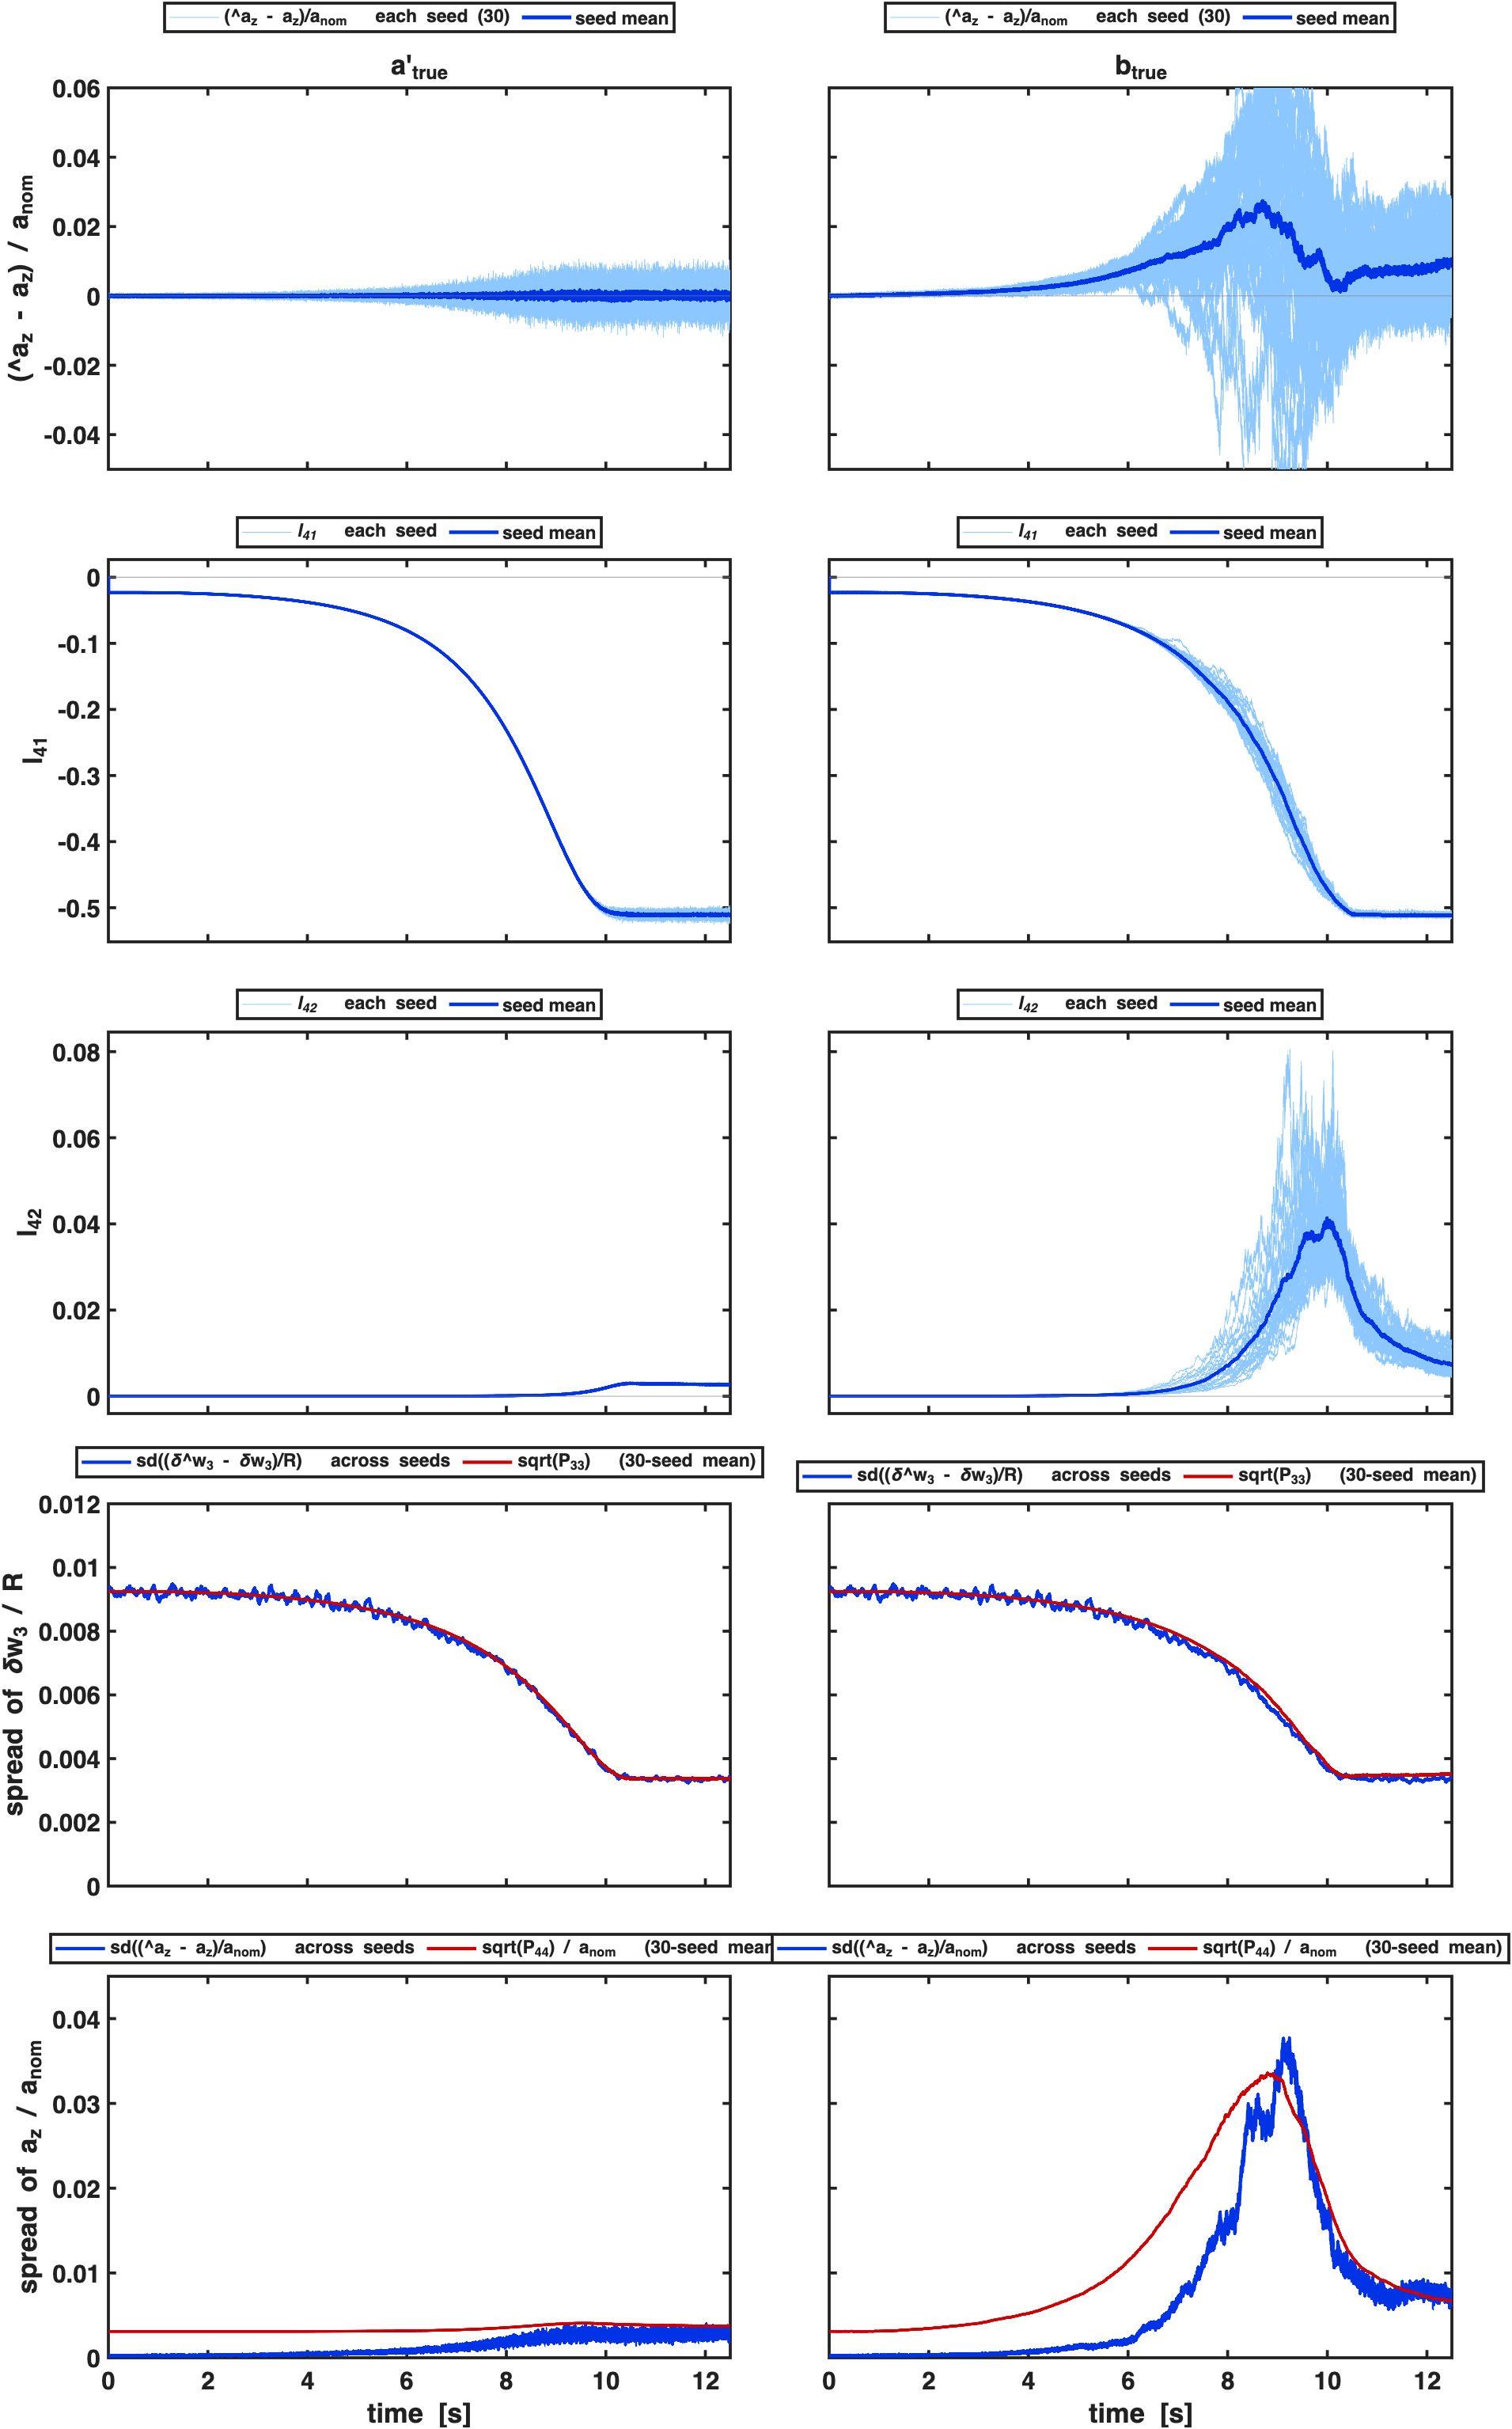
\includegraphics[width=\textwidth]{figures/arms30_seedtruth_pair.png}
\end{figure}

\end{document}
